In this lab we will be doing an offline password attack using a rainbow table.
Passwords are gathered from a Windows 10 VM using PwDump v8.2

First we create new user accounts with simple passwords.
\begin{figure}[H]
    \centering
    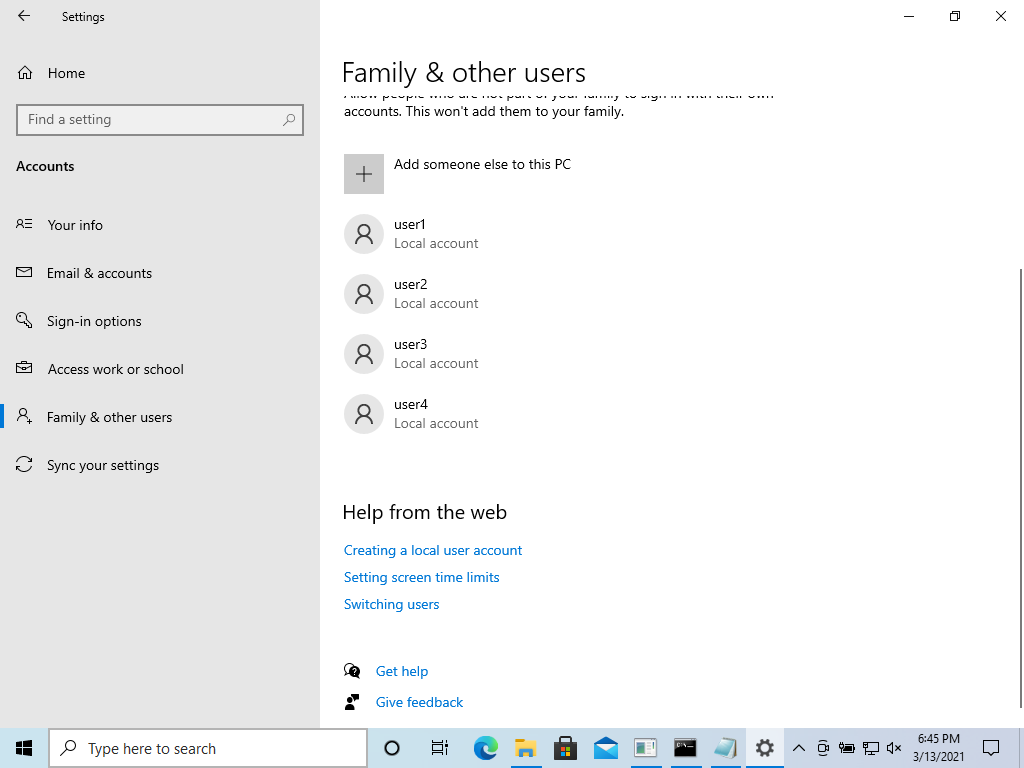
\includegraphics[width=\linewidth]{figures/1-users.png}
    \caption{List of users whose passwords will be cracked.}
\end{figure}

Next we install and run PwDump to retrieve the passwords hashes from the system files.
\begin{figure}[H]
    \centering
    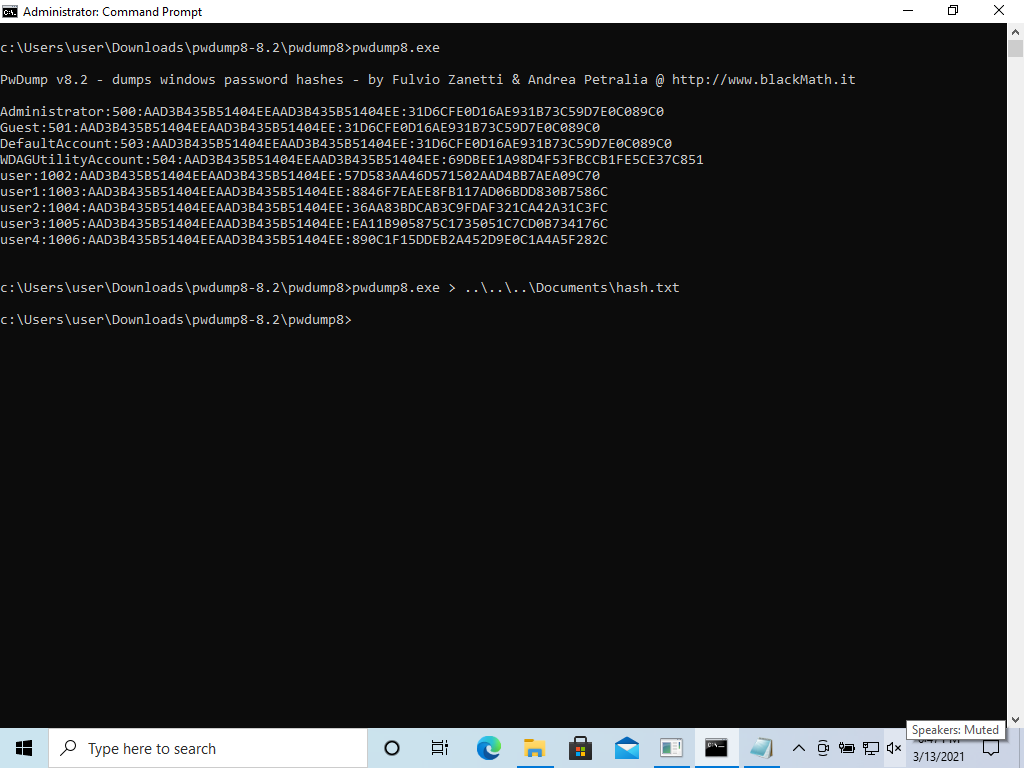
\includegraphics[width=\linewidth]{figures/2-pwdump.png}
    \caption{List of all users on the machine and their associated password hashes.}
\end{figure}

Now we generate a rainbow table to match the possible passwords.
\begin{figure}[H]
    \centering
    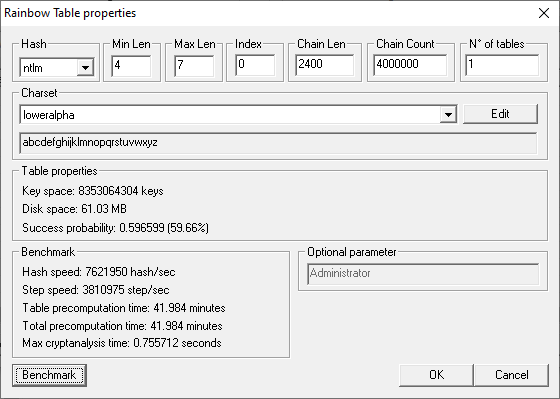
\includegraphics[width=\linewidth]{figures/3-create-rainbow-table.png}
    \caption{Parameters for creating the rainbow table.}
\end{figure}
\begin{figure}[H]
    \centering
    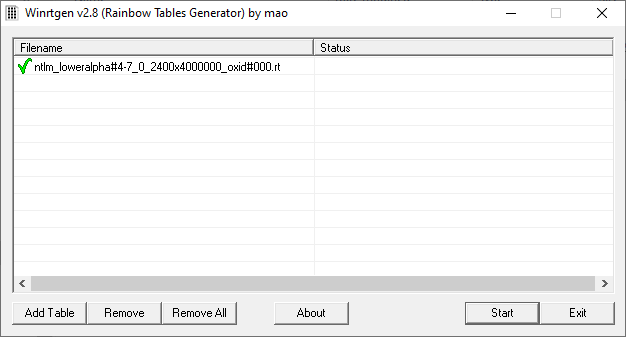
\includegraphics[width=\linewidth]{figures/4-rainbow-table-complete.png}
    \caption{Completed rainbow table.}
\end{figure}

RainbowCrack had an issue with finding the proper DLL's so I had to import them from my host machine.
Once RainbowCrack was working I added the hashes.
After locating the rainbow table, RainbowCrack will find the hashes.
\begin{figure}[H]
    \centering
    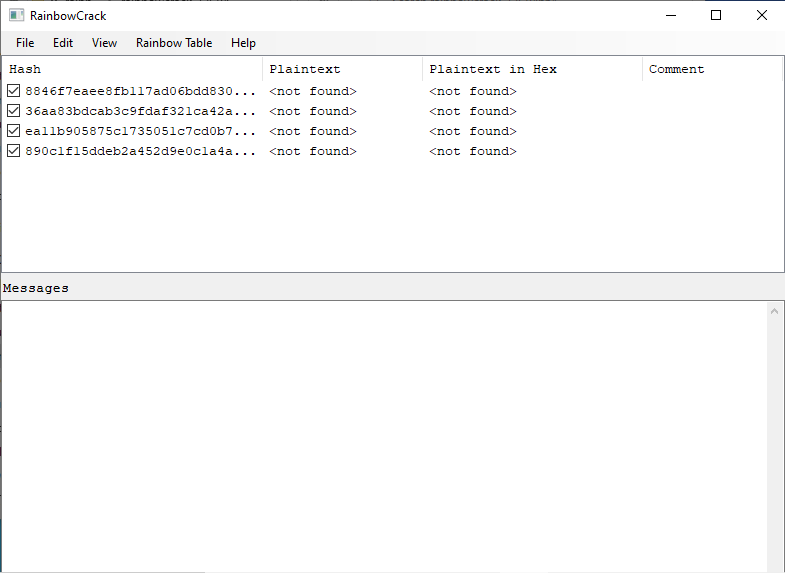
\includegraphics[width=\linewidth]{figures/5-add-hashes.png}
    \caption{Added hashes to RainbowCrack.}
\end{figure}
\begin{figure}[H]
    \centering
    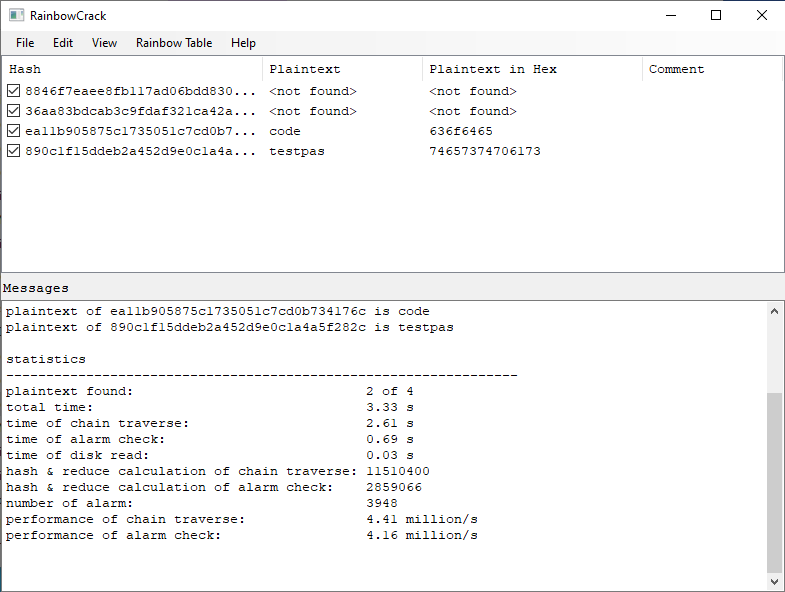
\includegraphics[width=\linewidth]{figures/6-crack-hashes.png}
    \caption{Output of RainbowCrack attempting to find the passwords.}
\end{figure}

I assume that the reason some passwords were not found was the the rainbow table we generated was not large enough.
As a separate test I took them to \verb|crackstation.net| and their rainbow table was able to find the passwords.
\begin{figure}[H]
    \centering
    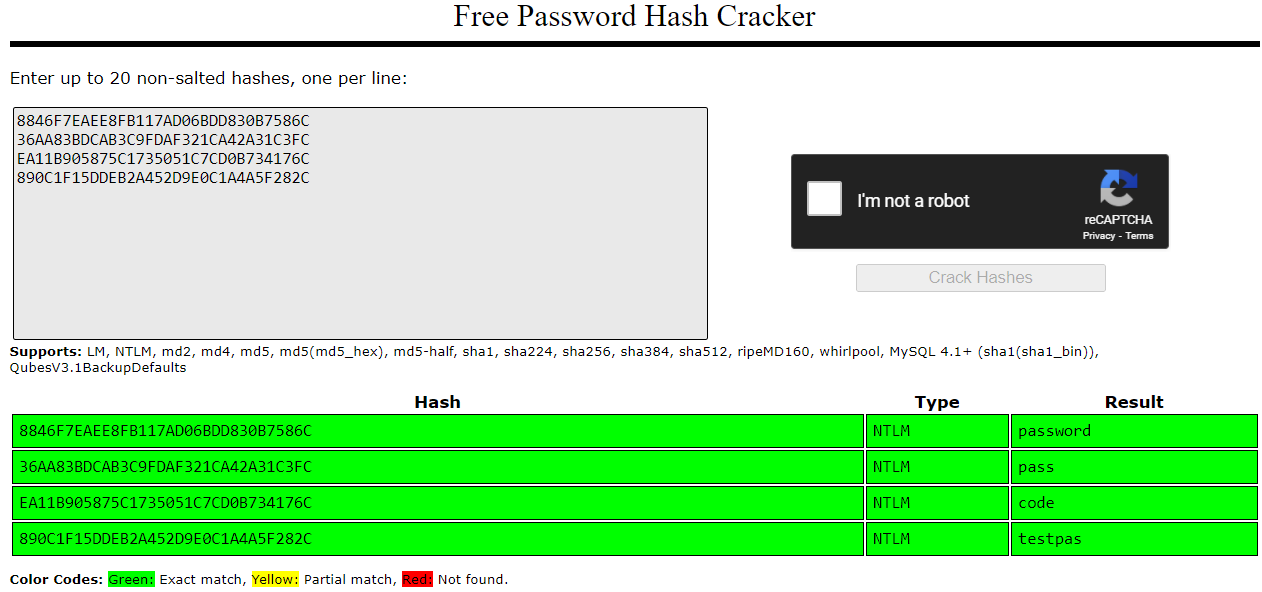
\includegraphics[width=\linewidth]{figures/7-crack-hash.png}
    \caption{CrackStation.net output.}
\end{figure}

This lab taught me how to crack passwords using a rainbow table.
First there need to be accounts with passwords susceptible to attacks.
These passwords are retrieved from the Security Account Manager (SAM) database file.
Next we create a rainbow table that fit the minimum needs of the passwords we are cracking.
As stated earlier, the number of values is probably to small to exhaust the password list.
RainbowCrack is used to compare the password hashes to the rainbow table, and print the initial text to create the hash.